% Opcje klasy 'iithesis' opisane sa w komentarzach w pliku klasy. Za ich pomoca
% ustawia sie przede wszystkim jezyk i rodzaj (lic/inz/mgr) pracy, oraz czy na
% drugiej stronie pracy ma byc skladany wzor oswiadczenia o autorskim wykonaniu.
\documentclass[declaration,shortabstract]{iithesis}

\usepackage[utf8]{inputenc}

%%%%% DANE DO STRONY TYTUŁOWEJ
% Niezaleznie od jezyka pracy wybranego w opcjach klasy, tytul i streszczenie
% pracy nalezy podac zarowno w jezyku polskim, jak i angielskim.
% Pamietaj o madrym (zgodnym z logicznym rozbiorem zdania oraz estetyka) recznym
% zlamaniu wierszy w temacie pracy, zwlaszcza tego w jezyku pracy. Uzyj do tego
% polecenia \fmlinebreak.
\polishtitle    {Aplikacja wizualizująca działanie\fmlinebreak transducerów Mealy'ego i Moore'a}
\englishtitle   {Mealy's and Moore's transducers visualizer}
\polishabstract {Celem pracy jest zaprezentowanie aplikacji wizualizującej model matematyczny zwany transducerem. Transducery są niezwykle przydatne przy przetwarzaniu języka i mowy \cite{Zastosowanie 2}. Dzięki zastosowaniu transducerów potrafimy często uprościć rozwiązania wielu problemów zaczynając od prostych problemów jak sprawdzanie palindromiczności słowa[Przykład \ref{parz_pal}], kończąc na zmianie struktury systemów rozpoznających mowę \cite{Zastosowanie 1}. }
\englishabstract{In this thesis we present the Transducer Visualizer application which is able to visualize mathematical model called transducer. Main purpose of using transducer is language and speach processing \cite{Zastosowanie 2}. Transducers can simplify and speed up solutions of many problems like palindrom checking [Example \ref{parz_pal}] or even speach recognition \cite{Zastosowanie 1}. }
% w pracach wielu autorow nazwiska mozna oddzielic poleceniem \and
\author         {Bartłomiej Najdecki}
% w przypadku kilku promotorow, lub koniecznosci podania ich afiliacji, linie
% w ponizszym poleceniu mozna zlamac poleceniem \fmlinebreak
\advisor        {dr Jakub Michaliszyn}
\date          {30 czerwca 2017}                     % Data zlozenia pracy
% Dane do oswiadczenia o autorskim wykonaniu
\transcriptnum {273975}                     % Numer indeksu
\advisorgen    {dr Jakuba Michaliszyna} % Nazwisko promotora w dopelniaczu
%%%%%

%%%%% WLASNE DODATKOWE PAKIETY
%
\usepackage{graphicx,listings,amsmath,amssymb,amsthm,amsfonts, sidecap, makecell, rotating}
%
%%%%% WŁASNE DEFINICJE I POLECENIA
\theoremstyle{definition}
\newtheorem{exmp}{Przykład}[section]
%\theoremstyle{definition} \newtheorem{definition}{Definition}[chapter]
%\theoremstyle{remark} \newtheorem{remark}[definition]{Observation}
\theoremstyle{plain} 
\newtheorem{theorem}{Twierdzenie}
%\theoremstyle{plain} \newtheorem{lemma}[definition]{Lemma}
%\renewcommand \qedsymbol {\ensuremath{\square}}
% ...
%%%%%

\begin{document}

%%%%% POCZĄTEK ZASADNICZEGO TEKSTU PRACY

\chapter{Wprowadzenie}
\section{Automat skończony}
Automat skończony (Deterministic Finite-state Automaton) jest modelem matematycznym systemu o dyskretnych wejściach i wyjściach \cite{Wprowadzenie do teorii}. Automaty najczęściej wykorzystuje się do sprawdzenia przynależności danego słowa do definiowanego przez nie języka. DFA jest 5 elementową krotką \(\langle \Sigma, Q,  q_0, F, \delta \rangle \), gdzie \(\sigma\) to alfabet nad którym język rozważamy, Q to zbiór stanów automatu, \(q_0\) - wyróżniony stan początkowy, F - podzbiór Q, oznaczający stany akceptujące oraz \(\delta\) - funkcja przejścia pomiędzy stanami, definiowana jako funkcja typu: 
$$ Q \times \Sigma \rightarrow Q$$
Automat odczytuje słowo litera po literze zmieniając stany przy użyciu funkcji przejśca, a następnie, w zależności od tego czy jest w stanie akceptującym czy nie, akceptuje bądź odrzuca słowo. Prosty przykład DFA jest ukazany na rysunku \ref{fig:obrazek DFA} - jest to automat akceptujący słowa, których sufiks to ABCD. Automat rozpoczyna w stanie A, a następnie zmienia stan na B, gdy odczyta A, natomiast w przeciwnym przypadku nie zmienia stanu. Stanem akceptującym jest X (nie zaznaczony). Sporą zaletą definiowanych w ten sposób automatów jest liniowa złożoność przetwarzania słów (zakładając, że automat już wcześniej został stworzony), jednak są to modele mocno ograniczone - języki przez nie rozpoznawane są bardzo proste. Języki rozpoznawalne przez automaty skończone nazywamy językami regularnymi.
Dla ułatwienia definiujemy rozszerzenie funkcji \(\delta\) w ten sposób:
$$ \hat\delta(q, a) = \delta(q, a) $$
$$ \hat\delta(q, wa) = \delta(\delta(w, q), a) $$
\begin{figure}
\centering
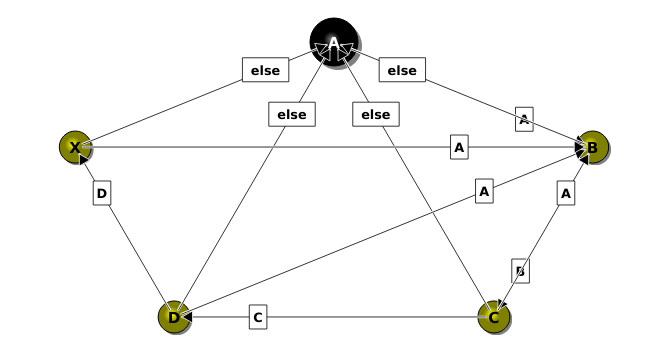
\includegraphics[width=\textwidth]{fsm.png}
\caption[caption]{Przykład DFA - na czarno zaznaczony wierzchołek początkowy.\\\hspace{\textwidth}Stanem akceptującym jest X}
\label{fig:obrazek DFA}
\end{figure}
\section{Automat skończony ze stosem}
Aby zwiększyć zbiór możliwych do rozpoznania języków dodamy do automatu stos - oprócz stanu, automat będzie miał stos będący skończonym słowem nad pewnym alfabetem \(\Sigma'\) z wyróżnionym znakiem \(k_{\Sigma'}\) oznaczającym dno stosu. Zmiany wymaga również funkcja przejścia:
$$ Q \times \Sigma \times \Sigma' \rightarrow  Q \times \Sigma^{'*}$$
Funkcja \( \delta \) zależy teraz również od tego co jest na szczycie stosu. Istnieją dwie konwencje akceptowania przez taki automat:
\begin{itemize}  
\item Przez pusty stos
\item Przez osiągniecie stanu akceptowalnego
\end{itemize}
W przypadku transducerów, które są tematem tej pracy, to rozróżnienie nie jest potrzebne (transducer nie akceptuje).
Dzięki takiemu rozszerzeniu klasa jęzków rozpoznawalnych przez automaty rozszerza się do języków bezkontektowych.
\section{Transducer Mealy'ego}
Automaty ze stosem są potężnym modelem matematycznym, jednak po\-tra\-fią 
one tylko rozstrzygać problem przynależności słowa do języka.
Automaty potrafią z łatwością znajdować wzorce w tekście 
- dlaczego miałyby nie umieć ich za\-stę\-po\-wać albo zliczać?\\
Transducerem Mealy'ego \cite{Mealy book} nazywamy krotkę 
$$ \langle \Sigma, \Sigma_1, Q, q_0, \delta, \sigma \rangle $$
w której \( \langle \Sigma, Q, q_0, \emptyset, \delta \rangle \) jest DFA z pustym zbiorem akceptującym, 
natomiast \(\sigma\) jest funkcją \(Q \times \Sigma \rightarrow \Sigma_1^{*} \). Dodatkowo dla transducera T definiujemy 
$$f_T(wa) = f_T(w)\sigma(\delta(w, q_0), a) $$
\(f_T\) jest funkcją wyjścia transducera - to za jej pomocą generujemy wynik działania transducera.
\begin{exmp}
Rozważmy problem wyszukiwania wzorca ABCD w tekście i zastępowania go wzorcem EF. Zdefiniujmy zbiór stanów w następujący sposób:
$$ Q = \{None, A, AB, ABC\} $$ 
Następnie definujemy deltę w ten sposób:
\begin{table*}[h]
    \centering
    \begin{tabular}{|c||c | c | c| c|}
        \hline       
          & None & A & AB & ABC \\ \hline \hline 
        a & A    & A & A  & A \\ \hline
        b & None & AB & None & None \\ \hline
        c & None & None & ABC & None \\ \hline
        inna & None & None & None & None\\  \hline
    \end{tabular} 
    \caption{Funkcja przejścia}
    \label{tab:my_label}
\end{table*}
\begin{figure*}[h]
\centering
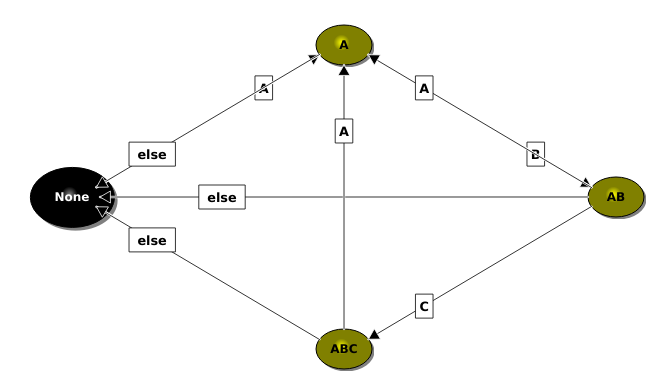
\includegraphics[width=\textwidth]{abc.png}
\caption{DFA należące do transducera}
\label{fig:abc}
\end{figure*} \\
Pozostało już tylko odpowiednio zdefiniować funkcję \(\sigma\). Chcemy, by \(\sigma\) nie wypisywała nic, gdy natrafi na kolejną literę wzorca lub wypisała EF gdy wzorzec się skończy, natomiast gdy wczytana litera nie jest kolejną literą wzorca funkcja powinna przepisać literę. Dla wygody oznaczmy przez \(\$\) literę wczytaną przez \(\sigma\):\\
\begin{table*}[h]
    \centering
    \begin{tabular}{|c||c | c | c| c|}
        \hline       
          & None & A & AB & ABC \\ \hline \hline 
        a & \(\epsilon\) & a & ab  & abc \\ \hline
        b & b & \(\epsilon\) & abb & abcb \\ \hline
        c & c & ac & \(\epsilon\) & abcc \\ \hline
        d & d & ad & abd & ef \\ \hline 
        inna & \$ & a\$ & ab\$ & abc\$\\  \hline
    \end{tabular} 
    \caption{Funkcja przejścia}
    \label{tab:my_label}
\end{table*}
Zdefiniowany w ten sposób transducer pamięta w stanie ile liter wyszukiwanego wzorca wczytał, by móc w odpowiednim momencie wypisać 'ef' lub wczytany prefiks wzorca.
\end{exmp}
\section{Transducer Moore'a}
Różnica pomiędzy transducerem Moore'a a Mealy'ego polega na innej definicji funkcji \(\sigma\)\cite{Moore book}. W transducerze Mealy'ego funkcja \(\sigma\) miała typ:
$$ Q \times \Sigma \rightarrow \Sigma_1^{*} $$
Natomiast w transducerze Moore'a \(\sigma\) jest funkcją:
$$ Q \rightarrow \Sigma_1^{*} $$
Poniższe twierdzenie jest znane z literatury (zobacz \cite{linz2011introduction}).
\begin{theorem}
\label{rownowaznosc transducerow}
Powyższe modele są równoważne. 
\end{theorem}
\begin{proof} 
Aby z transducera Moore'a zrobić transducer Mealy'ego wystarczy pomijać drugi parametr - niech \(\sigma_{Mo} \) oznacza funkcję \(\sigma\)  dla transducera Moore'a. Wtedy definiujemy \(\sigma_{Me}\) równoważnego transducera Mealy'ego jako:
$$ \sigma_{Me}(q, a) = \sigma_{Mo}(q) $$
Konwersja automatu Mealy'ego na automat Moore'a jest nieco bardziej skomplikowana. Niech \( \langle \Sigma, \Sigma_1, Q, q_0, \delta, \sigma \rangle \) oznacza pewien automat Mealy'ego. Chcemy znaleźć równoważny automat Moore'a \(\langle\Sigma', \Sigma_1', Q', q_0', \delta', \sigma'\rangle\). Z oczywistych powodów, wiemy że:
$$ \Sigma' = \Sigma $$
$$ \Sigma_1' = \Sigma_1 $$
Następnie zdefinujmy zbiór stanów \(Q'\):
$$ Q' = Q \times \Sigma $$
Teraz możemy pamiętać ostatnio wczytaną literę potrzebną funkcji \(\sigma\) w transducerze Mealy'ego.
$$ \delta'( (q,a), b) = (\delta(q,a), b) $$
$$ \sigma'( (q,a) ) = \sigma(q,a) $$
Poprawność wynika z konstrukcji.
\end{proof}
\section{Transducery ze stosem}
Wiedząc już co to są transducery bardzo łatwo możemy rozszerzyć ich definicję do transducerów ze stosem. Transducerem ze stosem nazwiemy krotkę 
$$ \langle \Sigma, \Sigma_1, \Sigma', Q, q_0, \delta, \sigma \rangle $$
w której \( \langle \Sigma, \Sigma', Q, \emptyset, q_0, \delta \rangle \) jest automatem skończonym ze stosem, zaś \(\sigma\) jest funkcją:
\begin{itemize}
\item \( Q \times \Sigma \times \Sigma' \rightarrow \Sigma^*_1 \) dla transducerów ze stosem Mealy'ego
\item \( Q \times \Sigma' \rightarrow \Sigma^*_1 \) dla transducerów Moore'a
\end{itemize}
Co więcej, również te transducery są równoważne (dowód taki sam jak w twierdzeniu [\ref{rownowaznosc transducerow}]).
\chapter{Aplikacja}
Link do repozytorium aplikacji \cite{Repo}. Znajduje się tam również dokładna instrukcja instalacji.
\section {Technologie}
\subsection{Biblioteka graficzna}
Aplikacja w całości została napisana w C++ wraz z biblioteką Qt. Qt jest zestawem przenośnych bibliotek dedykowanych C++ i Javie udostępnianych na licencji GPL, LGPL i komercyjnej. Jest to bardzo dojrzała biblioteka - pierwsza komercyjna wersja powstała w latach 90 \cite{qt link}. Obecnie jest to najpopularniejsza bibliteka dla aplikacji okienkowych w C++ dla systemu Linux - na Qt bazuje m.in. KDE. Dzięki temu aplikacja jest stabilna i przenośna. Do testowania aplikacji użyłem komponentu bibliteki Qt - QtTest.
\subsection{Format wejścia}
Transducery są wczytywane z plików o rozszerzeniu 'json' w formacie przypominającym uproszczonego JSON'a. Format JSON został wybrany ze względu na czytelność oraz łatwość opisu i rozbudowywania. Opis każego transducer'a musi zawierać wewnątrz klamr \{\}. Tablica \ref{tab:properties} opisuje pola, które powinien posiadać opis transducer.\\
\begin{table*}[h]
    \centering
    \begin{tabular}{|c|l|}
    \hline
        Nazwa pola & Znaczenie \\ \hline\hline
        \textbf{name} & Wyświetlana w programie nazwa transducera \\\hline
        \textbf{states} & \makecell[l]{Dyskretny zbiór stanów transducera \\ prezentowany w postaci grafu w aplikacji} \\\hline
        \textbf{initial\_state} & Stan początkowy\\\hline
        \textbf{type} & \makecell[l]{Ma wartość Mealy jeśli opisujemy transducer Mealy'ego.\\
                                     Ma wartość Moore jeśli opisujemy transducer Moore'a.} \\\hline
        \textbf{delta} & Funkcja przejścia DFA, więcej poniżej \\\hline
        \textbf{sigma} & Funkcja wyjścia transducera, więcej poniżej \\\hline
        hasStack & \makecell[l]{Jeśli ma wartość 'true' to transducer ma stos.\\
                            Jeśli pominiemy pole lub ustawimy na inną wartość,\\
                            to transducer nie będzie miał stosu}\\\hline
    \end{tabular}
    \caption{Lista właściwości transducera - pogrubione właściwości są obowiązkowe}
    \label{tab:properties}
\end{table*}
\pagebreak
Typ funkcji \(\sigma\) oraz \(\delta\) zależy od typu transducer - tabela \ref{tab:types}. W tej aplikacji opis \(\delta\) oraz \(\sigma\) wygląda w podobny sposób i przypomina konstrukcję switch-case - opisujemy przypadki pozbywając się kolejnych argumentów aż do usunięcia wszystkich akcji. Po przejściu przez wszystkie argumenty wykonujemy zapisaną akcję. Przykładowy opis znajduje się na obrazku \ref{fig:przykladowy_opis}. \\ 
\begin{table*}[h]
    \centering
    \begin{tabular}{|c|c|c|}
        \hline
        Type transducera & typ funkcji \(\delta\) & typ funkcji \(\sigma\) \\ \hline
        Transducer Mealy'ego bez stosu & \(Q \times \Sigma \rightarrow Q\) & \(Q \times \Sigma \rightarrow \Sigma_1^*\)\\ \hline
        Transducer Moore'a bez stosu & \(Q \times \Sigma \rightarrow Q\) & \(Q \rightarrow \Sigma_1^*\)\\ \hline
        Transducer Mealy'ego ze stosu & \(Q \times \Sigma \times \Sigma' \rightarrow Q\) & \(Q \times \Sigma \times \Sigma' \rightarrow \Sigma_1^*\)\\ \hline
        Transducer Moore'ego ze stosu & \(Q \times \Sigma \times \Sigma' \rightarrow Q\) & \(Q \times \Sigma' \rightarrow \Sigma_1^*\)\\ \hline
    \end{tabular}
    \caption{Typy funkcji w zależności od typu transducera}
    \label{tab:types}
\end{table*} \\
\begin{figure*}[h]
    \centering
    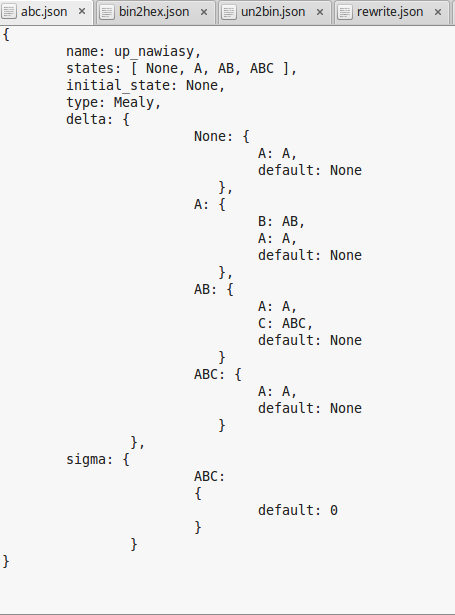
\includegraphics[width=10cm]{wejscie.png}
    \caption{Opis transducera zliczającego w systemie unarnym wystąpienia wzorca abc}
    \label{fig:przykladowy_opis}
\end{figure*}\\
Dodatkowo definujemy symbole specjalne 'default' lub równoważnie '\_' jako oznaczające dowolna inna wartość. Oprócz tego do dyspozycji mamy zarezerwowane słowo 'epsilon' oznaczające epsilon przejście. Jeśli epsilon występuje w miejscu wyboru wartości wczytanego symbolu, to nie powinien wystąpić żaden inny symbol (program zignoruje dodatkowy wybór)! W przypadku automatu ze stosem w miejscu selekcji górnego elementu stosu mamy do dyspozycji słowo 'empty', które oznacza pusty stos. \\
Przejdźmy teraz do opisu akcji, której wybór omówiliśmy powyżej. Akcje dla automatów bez stosu są opisane jako stan dla funkcji \(\delta\) lub jako słowo dla funkcji \(\sigma\). Dodatkowo funkcja \(\sigma\) podstawia za każde wystąpienie \$ wczytany znak (gdy akcja została wybrana jako default).\\
\pagebreak
Dla automatów ze stosem akcja jest opisana jako dwuelementowa lista - pierwszy element jest taki jak opisany powyżej, natomiast drugi jest poleceniem stosowym. Opis funkcji \(\sigma\) jest prawie taki sam - musimy dodać decyzję na podstawie stosu, dodatkowo każde wystąpienie \% zostanie zastąpione elementem ze szczytu stosu. Tablica \ref{tab:polecenia_stosowe} opisuje polecenia stosowe dla funkcji \(\delta\).\\
\begin{table*}[h]
    \centering
    \begin{tabular}{|c|c|}
    \hline
    Polecenie & Znaczenie \\ \hline
    vX     & Usuń X elementów ze stosu - X można pominąć (wtedy X=1). \\ \hline
    \(\wedge\)X     & \makecell{Dodaj litery słowa X na stos.\\Po dodaniu na szczycie stosu będzie ostatnia litera X.} \\ \hline
    \_ & Nic nie rób \\ \hline
    
    \end{tabular}
    \caption{Polecenia stosowe}
    \label{tab:polecenia_stosowe}
\end{table*}\\
\pagebreak
\section {Funkcjonalności}
\subsection{Pojedyńczy transducer}
Transducer jest prezentowany jako kolejno graf stanów z zaznaczonym aktualnym stanem, nazwą transducera, stosem wyświetlającym maksymalnie 12 elementów znajdujących się na szczycie, listą wczytanych znaków oraz aktualnym wyjściem transducera. Każdy transducer może zostać wczytany z pliku - więcej w następnej sekcji.
\subsection {Kolejka transducerów}
W celu uproszczenia rozwiązań zaimplementowałem kolejkę transducerów - wyjście każdego kolejnego transducera jest traktowane jako wejście kolejnego.\\ 
Aby dodać wierzchołek do listy wystarczy wybrać opcję 'Add to pipe' z menu 'Pipe' lub wcisnąć 'T'. W ten sposób dodajemy transducer z pliku. Nowo dodany transducer zostanie dodany do zakładek pod górnym menu programu. Aby zobaczyć jego składowe wystarczy kliknąć na zakładkę z jego nazwą.\\
Aby usunąć transducer musimy przełączyć widok za pomocą zakładek na transducer, który chcemy usunąć. Następnie z menu 'Pipe' wybieramy opcję 'Remove transducer'.\\
Aby ustawić wejście dla kolejki wystarczy wybrać 'Edit input' z menu 'Pipe' lub nacisnąć klawisz 'I'.  Symulację można uruchamiać na dwa sposoby:
\begin{itemize}
\item Tryb krokowy
\item Tryb normalny
\end{itemize}
W przypadku gdy wszystkie wejścia się wyczerpią aplikacja zakończy symulację.
W trybie krokowym, aplikacja wykonuje jeden krok. Aby wykonać kolejny krok należy wybrać opcję 'Next step' z menu transducer. Aplikacja dodatkowo przełącza pokazywany transducer na ten w którym został wykonany krok. Stan w którym aktualnie znajduje się transducer jest zaznaczony jako duży czarny wierzchołek, natomiast stan poprzedni jest zaznaczony jako mały, czarny wierzchołek. Aby uruchomić tryb krokowy wystarczy nacisnąć f10 lub wybrać opcję 'Step forward' z menu 'Pipe'.
W trybie normalnym aplikacja natychmiast wykona wszystkie możliwe kroki, a następnie przełączy widok na ostatni transducer, który wykonał akcję. Aby uruchomić tryb normalny wystarczy nacisnąć f5 lub wybrać opcję 'Run' z menu 'Pipe'.
\subsection{Widok}
\begin{figure*}[h]
\centering
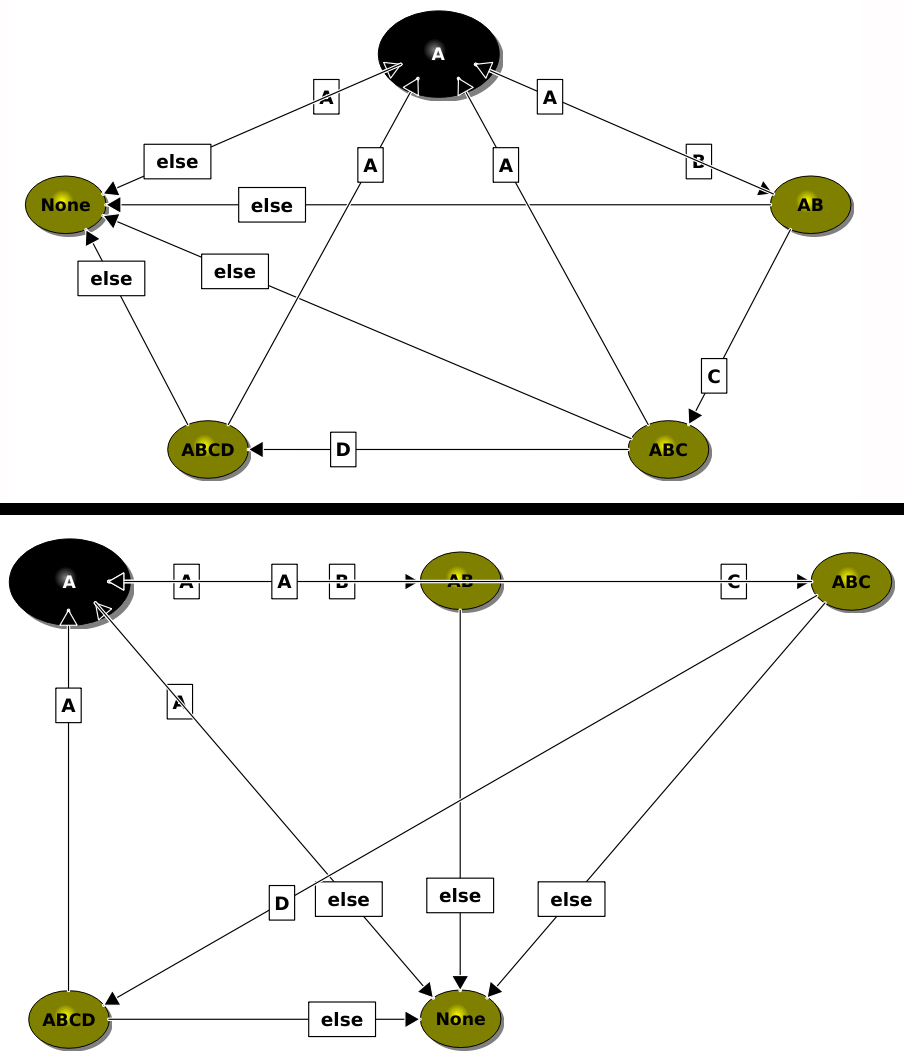
\includegraphics[width=\textwidth]{comp.png}
\caption{Porównanie rozmieszczenia na siatce i w wierzchołkach wielokąta foremnego}
\label{fig:comp}
\end{figure*}
Aplikacja wyświetla aktualny stan FSM należącego do transducera. Widok ten możemy przybliżać/oddalać za pomocą klawisza +/- lub wybierając odpowiednie opcje w menu View. Dodatkowo widok można przewijać za pomocą klawiszy W, S, A, D - bardzo przydatna opcja w przypadku analizy dużych transducerów.\\
Dodatkowo zaimplementowałem 3 proste algorytmy organizujące FSM:
\begin{itemize}
\item Organizuj w linii
\item Organizuj na siatce
\item Organizuj na wielokącie
\end{itemize}
Aby użyć algorytmu wystarczy wybrać odpowiednią opcję z zakładki 'Transducer'. Dla małych FSM z małymi stopniami wierzchołków najlepsze jest rozłożenie stanów jako wierzchołki wielokąta foremnego. W przypadku większych FSM świetnie sprawdza się rozkładanie ich na planie siatki. Dodatkowo każdy z wierzchołków może zostać przesunięty na dowolną pozycję przy pomocy myszki.
\section {Przykłady}
\subsection{Konwersja z systemu unarnego na system binarny}
Konwersja liczb ograniczonych przez pewną stałą N z systemu unarnego na system binarny, może odbyć się w prosty sposób za pomocą pojedyńczego transducer'a posiadającego liniową liczbę stanów, jednak nie jest rozwiązanie efektywne pamięciowo. Prezentowane tu rozwiązanie, używa 6 transducerów posiadających po 4 stany dla konwersji liczb nie większych niż \(2^6)\) z systemu unarnego do systemu dwójkowego - w ogólności potrzebujemy \(log(N) \) transducerów by przekonwertować liczby z systemu unarnego do systemu binarnego. Oto opis pojedyńczego transducera wraz z wizualizacją stanów:
\begin{figure*}[p]
\centering
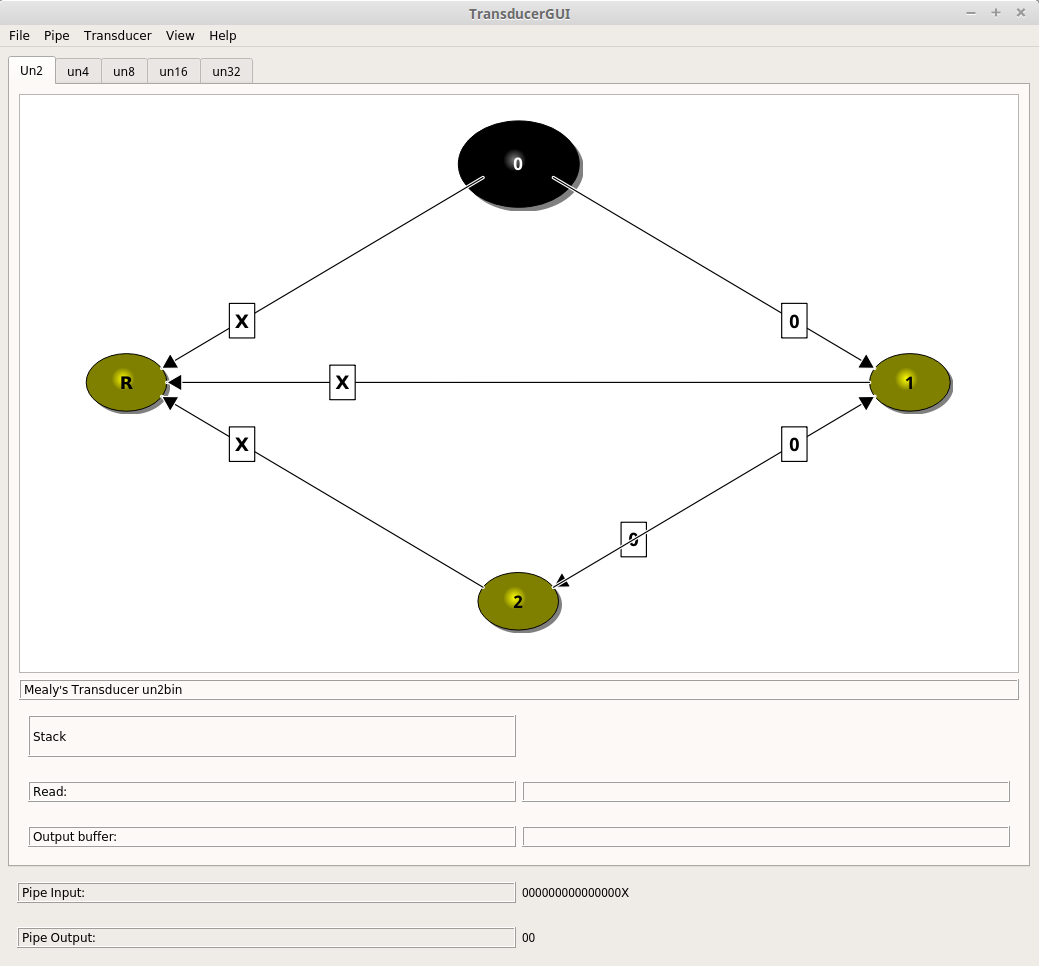
\includegraphics[width=\textwidth]{un2bin.png}
\caption{DFA należące do transducera konwertujące z systemu unarnego na binarny}
\label{fig:abc}
\end{figure*}
Dokładny opis transducer'a jest zapisany w katalogu Samples jako 'un2bin.json'. Aby przekonwertować daną liczbę musimy wpisać ją w systemie unarnym, a następnie napisać X jako znak końca liczby. Każdy transducer odczytuje postać unarną liczby, by następnie dopisać kolejny bit liczby w systemie binarnym i przepisać wcześniej obliczone już bity. Dodatkowo, każdy transducer skraca zapis unarny liczby dwukrotnie - dlatego potrzebujemy jedynie \(log(N)\) transducerów. Za zmniejszoną złożoność pamięciową płacimy złożonością czasową - transducer wykonuje \(log(N)\) przetworzeń wejścia. Widać, że w podobny sposób można stworzyć transducer konwertujący z dowolnego systemu liczbowego na dowolny inny w znacznie mniejszej niż liniowa pamięci.
\subsection{Korekta literówek}
Transducery najczęściej są używane do przetwarzania języków. Prostym przykładem transducerów może być aplikacja poprawiająca popularne błędy językowe. W tym przykładzie transducer poprawia dwa popularne błędy językowe:
\begin{itemize}
\item napewno \(\rightarrow\) na pewno
\item nielada \(\rightarrow\) nie lada
\end{itemize}
Model FSM ze względu na swój rozmiar znajduje się na następnej stronie. Dokładny opis przykładu został zapisany w katalogi Samples pod nazwą 'corrector.json'. Transducer wyszukuje jednego z wzorców z bazy, a następnie próbuje go zastąpić. Jeśli w trakcie przetwarzania, któryś z wzorców przestaje pasować wypisujemy wczytane znaki. Zaletą tego rozwiązania jest mała złożoność pamięciowa i czasowa - złożoność pamięciowa jest liniowa względem sumy długości wszystkich wzorców w słowniku, natomiast czasowa jest liniowa względem długości wczytywanego tekstu.

\subsection{Proste wykrywanie parzystych palindromów}
\label{parz_pal}
Transducery mogą być również wykorzystywane do upraszczania rozwiązań. Oto prosty przykład rozwiązywania problemu palindromów. Rozwiązanie korzysta z trzech transducerów. Pierwszy z nich oblicza połowę długości słowa w systemie unarnym, a następnie przepisuje słowo, oddzielając je specjalnym znakiem @. Kolejny transducer przepisuje słowo wstawiając w środku słowa znak @. Ostatni transducer dodaje kolejne litery na stos, a gdy osiągnie znak @ zaczyna porównywać litery ze stosu z literami słowa. W ten sposób potrafimy deterministycznie znaleźć środek, by następnie móc deterministycznie zweryfikować palindromiczność. Słowo musi zostać podane w postaci 'kandydat\_na\_palindrom@@'. Transducery są zapisane odpowiednio jako pliki 'count\_and\_reverse.json', 'find\_center.json' i 'palindromChecker.json' w katalogu 'Samples'.
\begin{figure*}[h]
\centering
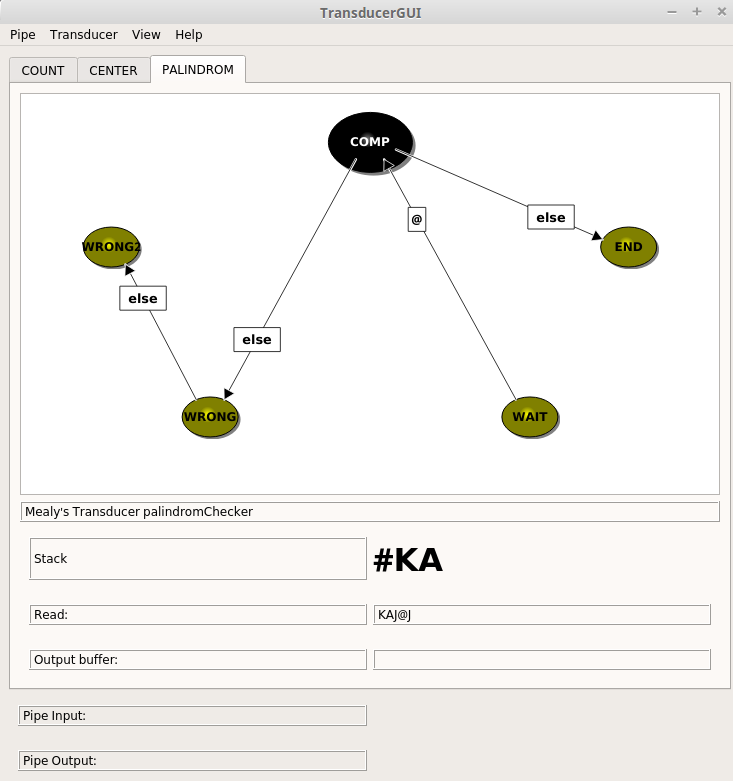
\includegraphics[width=\textwidth]{palindrom.png}
\caption{Ostatni transducer w kolejce sprawdzający palindromiczność początkowego słowa}
\label{fig:palindrom}
\end{figure*}
\begin{sidewaysfigure}[p]
\centering
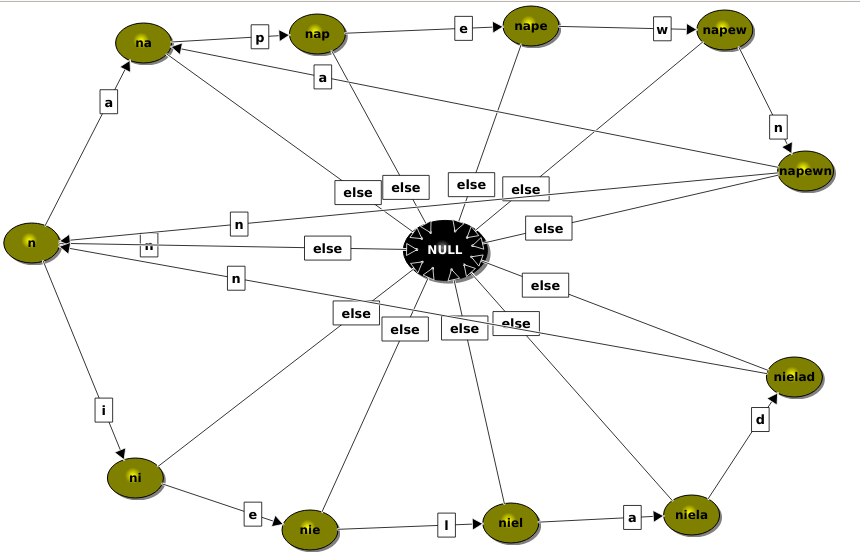
\includegraphics[width=\textwidth,height=\textheight,keepaspectratio]{correctorFSM.png}
\caption{DFA korektora językowego}
\label{fig:abc}
\end{sidewaysfigure}
\chapter{Podsumowanie}
\section{Zastosowania}
Transducery mają wiele zastosowań w przetwarzaniu języka. Jednym z głównych zastosowań jest użycie ich w przetwarzaniu mowy \cite{Zastosowanie 2}. Dzięki skończonemu automatowi stanowemu mogą opisywać lokalne w gramatyce zjawiska w przystępnej formie - do pełnej analizy i korekty potrzebne są graficzne narzędzia. Kolejnym argumentem przemawiającym za użyciem transducerów jest efektywność - czas działania nie zależy od wielkości transducera, lecz od wielkości wejścia.  Jednym z ciekawszych zastosowań jest użycie transducerów z wagami do reprezentacji ukrytych sieci Markova \cite{Zastosowanie 1}. Poza pracami naukowymi, transducery zostały użyte w systemie rozpoznającym mowę stworzonym przez North American Business News \cite{Zastosowanie 1}. Dzięki użyciu transducerów uzyskano rozwiązanie działające w czasie rzeczywistym, zajmujące niewiele więcej pamięci niż rozwiązanie korzystające z trigramów.
\section{Dalszy rozwój}
Ponieważ transducery są oparte na automatach skończonych można bardzo łatwo rozszerzać je o wszelkie mechanizmy z FSM, m.in.:
\begin{itemize}
\item transducery niedeterministyczne
\item transducery operujące na drzewach zamiast słów
\item transducery operujące na słowach skończonych
\item transducery z wagami
\end{itemize}
Aby aplikacja stała się wygodniejsza, powinna zostać dodatkowo zaimplentowana funkcjonalność tworzenia projektów - każdorazowe dodawanie transducerów do kolejki oraz ustawianie wierzchołków w czytelnych miejscach nie jest wygodne. Ponieważ wszystko jest zapisywane w formacie JSON, implementacja tego rozwiązania nie powinna być skomplikowana.
%%%%% BIBLIOGRAFIA

\begin{thebibliography}{10}
\bibitem{Repo} \emph{Repozytorium aplikacji} https://github.com/bartek1912/transducerVisualizer
\bibitem{Wprowadzenie do teorii} \emph{Wprowadzenie do teorii automatów, języków i obliczeń}. John E. Hopcroft, Jeffrey D. Ullman
\bibitem{Zastosowanie 1} \emph{Weighted finite-state transducers in speech recognition}. Mehryar Mohri, Fernando Pereira and Michael Riley
\bibitem{Zastosowanie 2} \emph{Finite-State Transducers in Language and Speech Processing}. Mehryar Mohri
\bibitem{qt link} \emph{Opis projektu QT} https://www.qt.io/company/
\bibitem{Mealy book} \emph{A Method for Synthesizing Sequential Circuits.} Mealy, George H. (1955)
\bibitem{Moore book} \emph{Gedanken-experiments on Sequential Machines}. Moore, Edward F (1956)
\bibitem{linz2011introduction}\emph{An introduction to formal languages and automata}.
  Linz, Peter, (2011)
\end{thebibliography}

\end{document}